\section{Skip Connections and U-Net}
\begin{frame}{}
    \LARGE Image Segmentation: \textbf{Skip Connections and U-Net}
\end{frame}

\begin{frame}{Can We Do Better?}
\begin{itemize}
    \item The downsampling-then-upsampling approach works well for semantic segmentation.
    \item \textbf{But... can we do better?}
    \item \textbf{Problem}: Important details and spatial information may be lost during downsampling.
    \pause
    \item \textbf{Solution}: Introduce \textbf{skip connections} between encoder and decoder to preserve spatial information.
\end{itemize}
\end{frame}

\begin{frame}{Skip Connections in Segmentation}
\begin{itemize}
    \item Directly connect features from downsampling layers to upsampling layers.
    \item Help recover lost spatial details and improve segmentation accuracy.
\end{itemize}
\begin{figure}
    \centering
    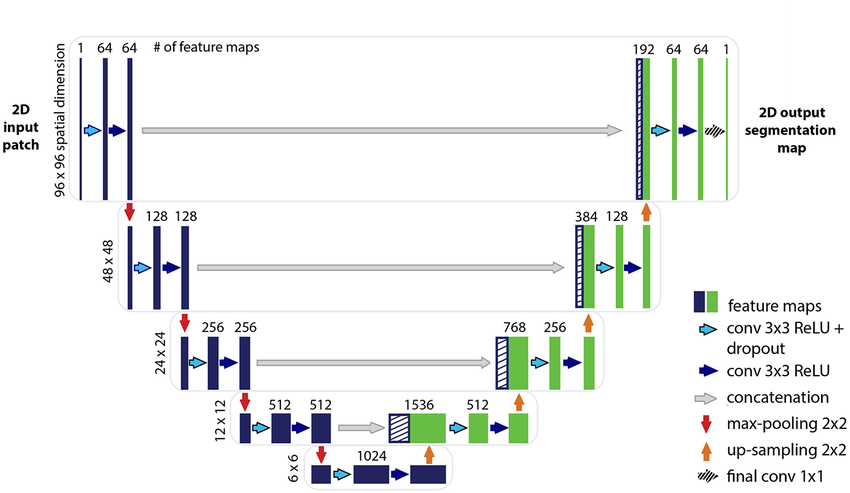
\includegraphics[width=1.0\textwidth,height=0.62\textheight,keepaspectratio]{images/segmentation/Unet.png}
    \caption*{\scriptsize Encoder-decoder with concatenation skip connections. Source: Livne et al., \emph{Front.\ Neurosci.} 13:97, 2019, Fig.~2 (CC BY).}
\end{figure}
\end{frame}

\begin{frame}{Skip Connections in Segmentation}
\begin{itemize}
    \item There are two types of skip connection (additive skips are what ``residual'' specifically means):
    \begin{itemize}
        \item \textbf{Addition:} Adds features from the encoder to the decoder \textbf{element-wise}.
        \item \textbf{Concatenation:} Concatenates features from the encoder to the decoder along the \textbf{channel dimension}.
    \end{itemize}
    \item \textbf{Which Is Better?}
    \begin{itemize}
        \item Concatenation is often better because it retains more feature information from the encoder.
        \item \textbf{Note}: addition requires the encoder and decoder features to match exactly in both spatial size and channel count; concatenation only needs spatial alignment, but increases the decoder's channel count.
    \end{itemize}
\end{itemize}
\end{frame}

\begin{frame}{U-Net}
\begin{itemize}
    \item This architecture, with concatenation skip connections, is called \textbf{U-Net}.
    \item \textbf{Why the name?}
    \begin{itemize}
        \item The architecture resembles the shape of the letter ``U''.
        \item Features are downsampled in the encoder and upsampled in the decoder, with skip connections in between.
    \end{itemize}
    \item U-Net is widely used for segmentation tasks, especially in biomedical imaging.
\end{itemize}
\begin{figure}
    \centering
    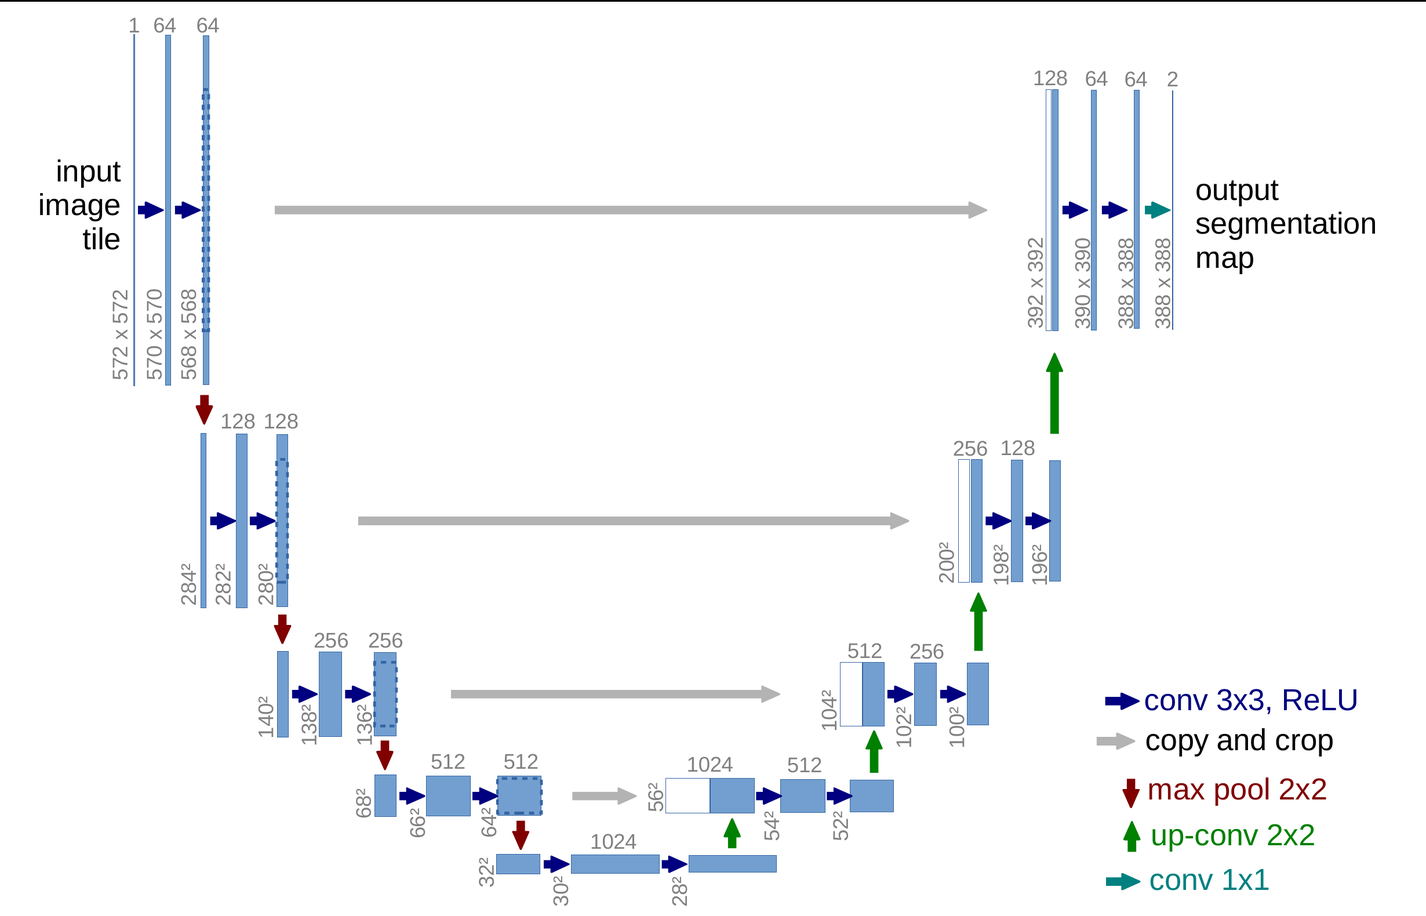
\includegraphics[width=0.72\linewidth,height=0.38\textheight,keepaspectratio]{images/segmentation/unet_architecture_ronneberger.png}
    \caption*{\scriptsize Source: Ronneberger, Fischer \& Brox, MICCAI 2015, Fig.~1.}
\end{figure}
\end{frame}

\begin{frame}{Using a Pretrained U-Net}
\begin{itemize}
    \item \textbf{Pretrained Encoder:}
    \begin{itemize}
        \item The encoder can use a pretrained backbone (e.g., ResNet, EfficientNet).
        \item This helps utilize features learned on large datasets (e.g., ImageNet).
        \item Only the decoder is trained from scratch for segmentation-specific tasks.
    \end{itemize}
\end{itemize}
\begin{figure}
    \centering
    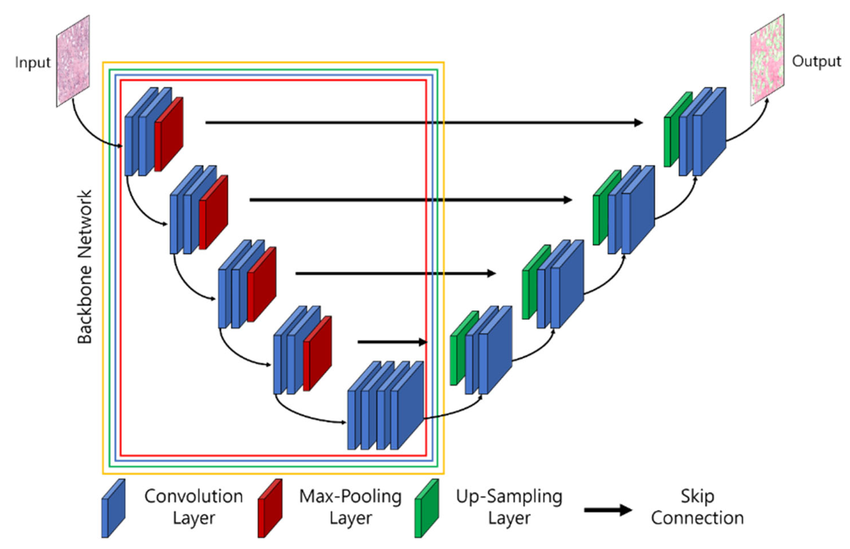
\includegraphics[width=0.55\linewidth,height=0.53\textheight,keepaspectratio]{images/segmentation/pretrained_unet.png}
    \caption*{\scriptsize Source: Ikromjanov et al., \emph{Cancers} 15(3):762, 2023, Fig.~5 (CC BY).}
\end{figure}
\end{frame}
